\chapter{Test Data Out Multiplexer (TDO MUX)}
\label{chap:tdo-mux}

This chapter gives an overview of TDO MUX and their operation. It contains the following sections:
\begin{itemize}
    \item \hyperref[sec:about-tdo-mux]{About TDO MUX}
\end{itemize}

\newpage

\section{About TDO MUX}
\label{sec:about-tdo-mux}
Based on the instruction selected by instruction decoder, The TDO MUX Block multiplexes the shifted bit from instruction register and data register to TDO in the negedge of TCK if no TRST is there else TDO gets 1’b0 value.

\vspace{1cm}
\begin{figure}[H]
    \centering
    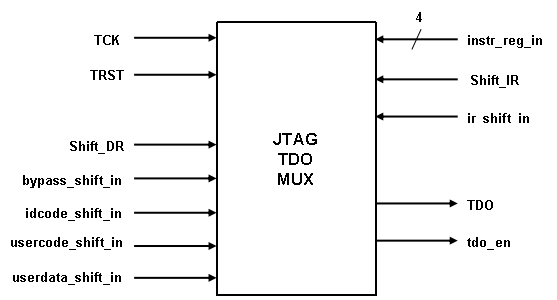
\includegraphics[width = 10cm]{images/jtag_tdo_mux.png}
    \vspace{1cm}
    \caption{JTAG Test data Output MUX}
    \label{fig:tdo-mux}
\end{figure}
\vspace{1cm}

\begin{longtable}{l l p{9.5cm}}
    \caption{TDO MUX port description}
    \label{tab:itdo-mux-ports}\\
    \hline
         \textbf{Port Name} & \textbf{Direction} & \textbf{Description}\\ \hline \hline
         \hyperref[subsec:tck]{TCK} & Input & Test Clock Input updates the data in the negedge of TCK.\\ \hline
        \hyperref[subsec:trst]{TRST} & Input & Asynchronous Active low reset that selects IDCODE Instruction by default. \\ \hline
        instr\_reg\_in & Input & Instruction coming from Instruction Register.
        
        \textbf{C1}: \texttt{instr\_reg\_in = bypass}, TDO gets bypass\_shift\_in
        
        \textbf{C2}: \texttt{instr\_reg\_in = idcode}, TDO gets idcode\_shift\_in
        
        \textbf{C3}: \texttt{instr\_reg\_in = usercode}, TDO gets usercode\_shift\_in
        
        \textbf{C4}: \texttt{instr\_reg\_in = userdata}, TDO gets userdata\_shift\_in
        
        The default case is bypass instruction. \\ \hline
        Shift\_IR & Input & If asserted, shifts the ir\_shift\_in to TDO in the negedge of TCK. \\ \hline
        ir\_shift\_in & Input & Instruction shift bit coming from Instruction Register.\\ \hline
        Shift\_DR & Input & If asserted, shifts the data bit to TDO in the negedge of TCK.\\ \hline
        bypass\_shift\_in & Input & bypass shift bit from Bypass Register. \\ \hline
        idcode\_shift\_in & Input & idcode shift bit from IDCODE Register.\\ \hline
        usercode\_shift\_in & Input & usercode shift bit from USERCODE Register.\\ \hline
        userdata\_shift\_in & Input & userdata shift bit from USERDATA Register. \\ \hline
        \hyperref[subsec:tdo]{TDO} & Output & Test Data Output.\\ \hline
        tdo\_en & Output & TDO enable signal asserted, if the state is either in the Shift\_IR or Shift\_DR State.\\ \hline
\end{longtable}